\section{序論}

社会ネットワーク分析は，人々の関係性を定量的に理解するための重要な手法である．
本レポートでは，ある集団における友人関係ネットワークを対象に，
6ヶ月間でどのような構造変化が生じたかを分析する．

分析にはネットワーク可視化・分析ツールであるCytoscapeを使用し，
入次数中心性，媒介中心性，近接中心性などの指標を算出した．
また，性別やグループといった属性に基づくネットワークパターンの可視化も行った．

\section{データ概要}

\subsection{ネットワークの基本情報}

分析対象のネットワークは，6ヶ月前（Before）と6ヶ月後（After）の2時点で取得された
友人関係データである．各ノードは個人を表し，エッジは友人関係を示す有向グラフである．

表\ref{tab:network_overview}に両時点のネットワーク基本統計を示す．

\begin{table}[htbp]
\centering
\caption{ネットワーク基本統計}
\label{tab:network_overview}
\begin{tabular}{lcc}
\toprule
指標 & Before & After \\
\midrule
ノード数 & 37 & 41 \\
エッジ数 & 46 & 67 \\
平均隣接ノード数 & 2.16 & 2.83 \\
ネットワーク直径 & 4 & 5 \\
特性経路長 & 1.93 & 2.27 \\
クラスタ係数 & 0.091 & 0.177 \\
ネットワーク密度 & 0.035 & 0.041 \\
連結成分数 & 6 & 2 \\
\bottomrule
\end{tabular}
\end{table}

\subsection{ノード属性}

各ノードには以下の属性が付与されている：
\begin{itemize}
  \item \textbf{ID}: 個人識別番号
  \item \textbf{グループ}: 1〜4の4グループ
  \item \textbf{性別}: 男性(m)または女性(f)
\end{itemize}

ノードラベルは「ID-グループ(性別)」の形式で表現される．
例えば「23-1(f)」はID:23，グループ1，女性を意味する．

図\ref{fig:network_before}および図\ref{fig:network_after}に，
それぞれBefore・Afterのネットワーク全体像を示す．

\begin{figure}[htbp]
\centering
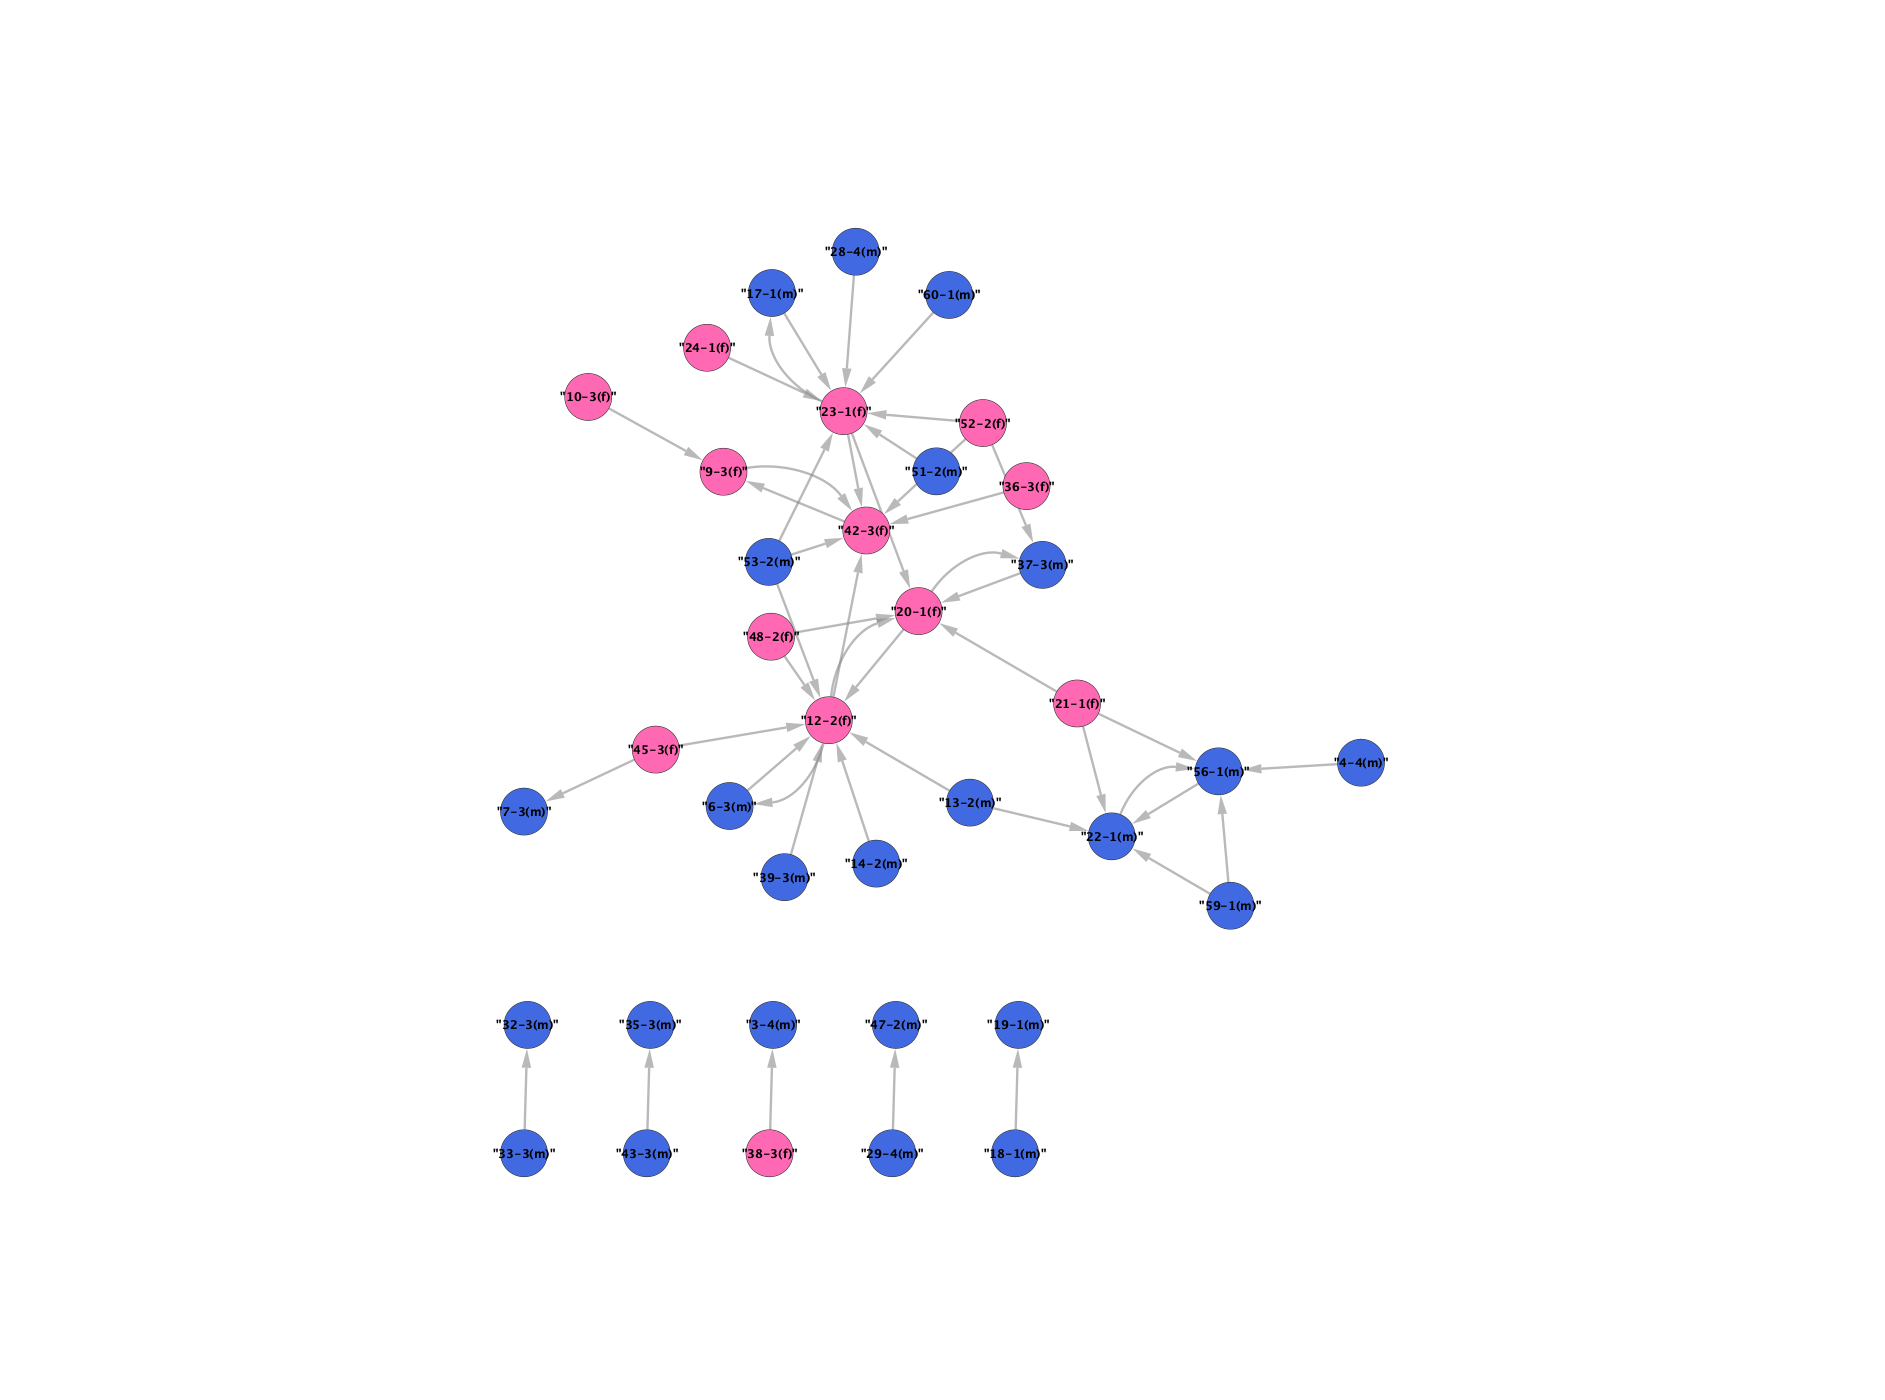
\includegraphics[width=0.95\linewidth]{fig/network_before.png}
\caption{Beforeネットワーク（6ヶ月前）．ノード色は性別を示す（ピンク：女性，青：男性）．矢印は友人関係の方向を表す．}
\label{fig:network_before}
\end{figure}

\begin{figure}[htbp]
\centering
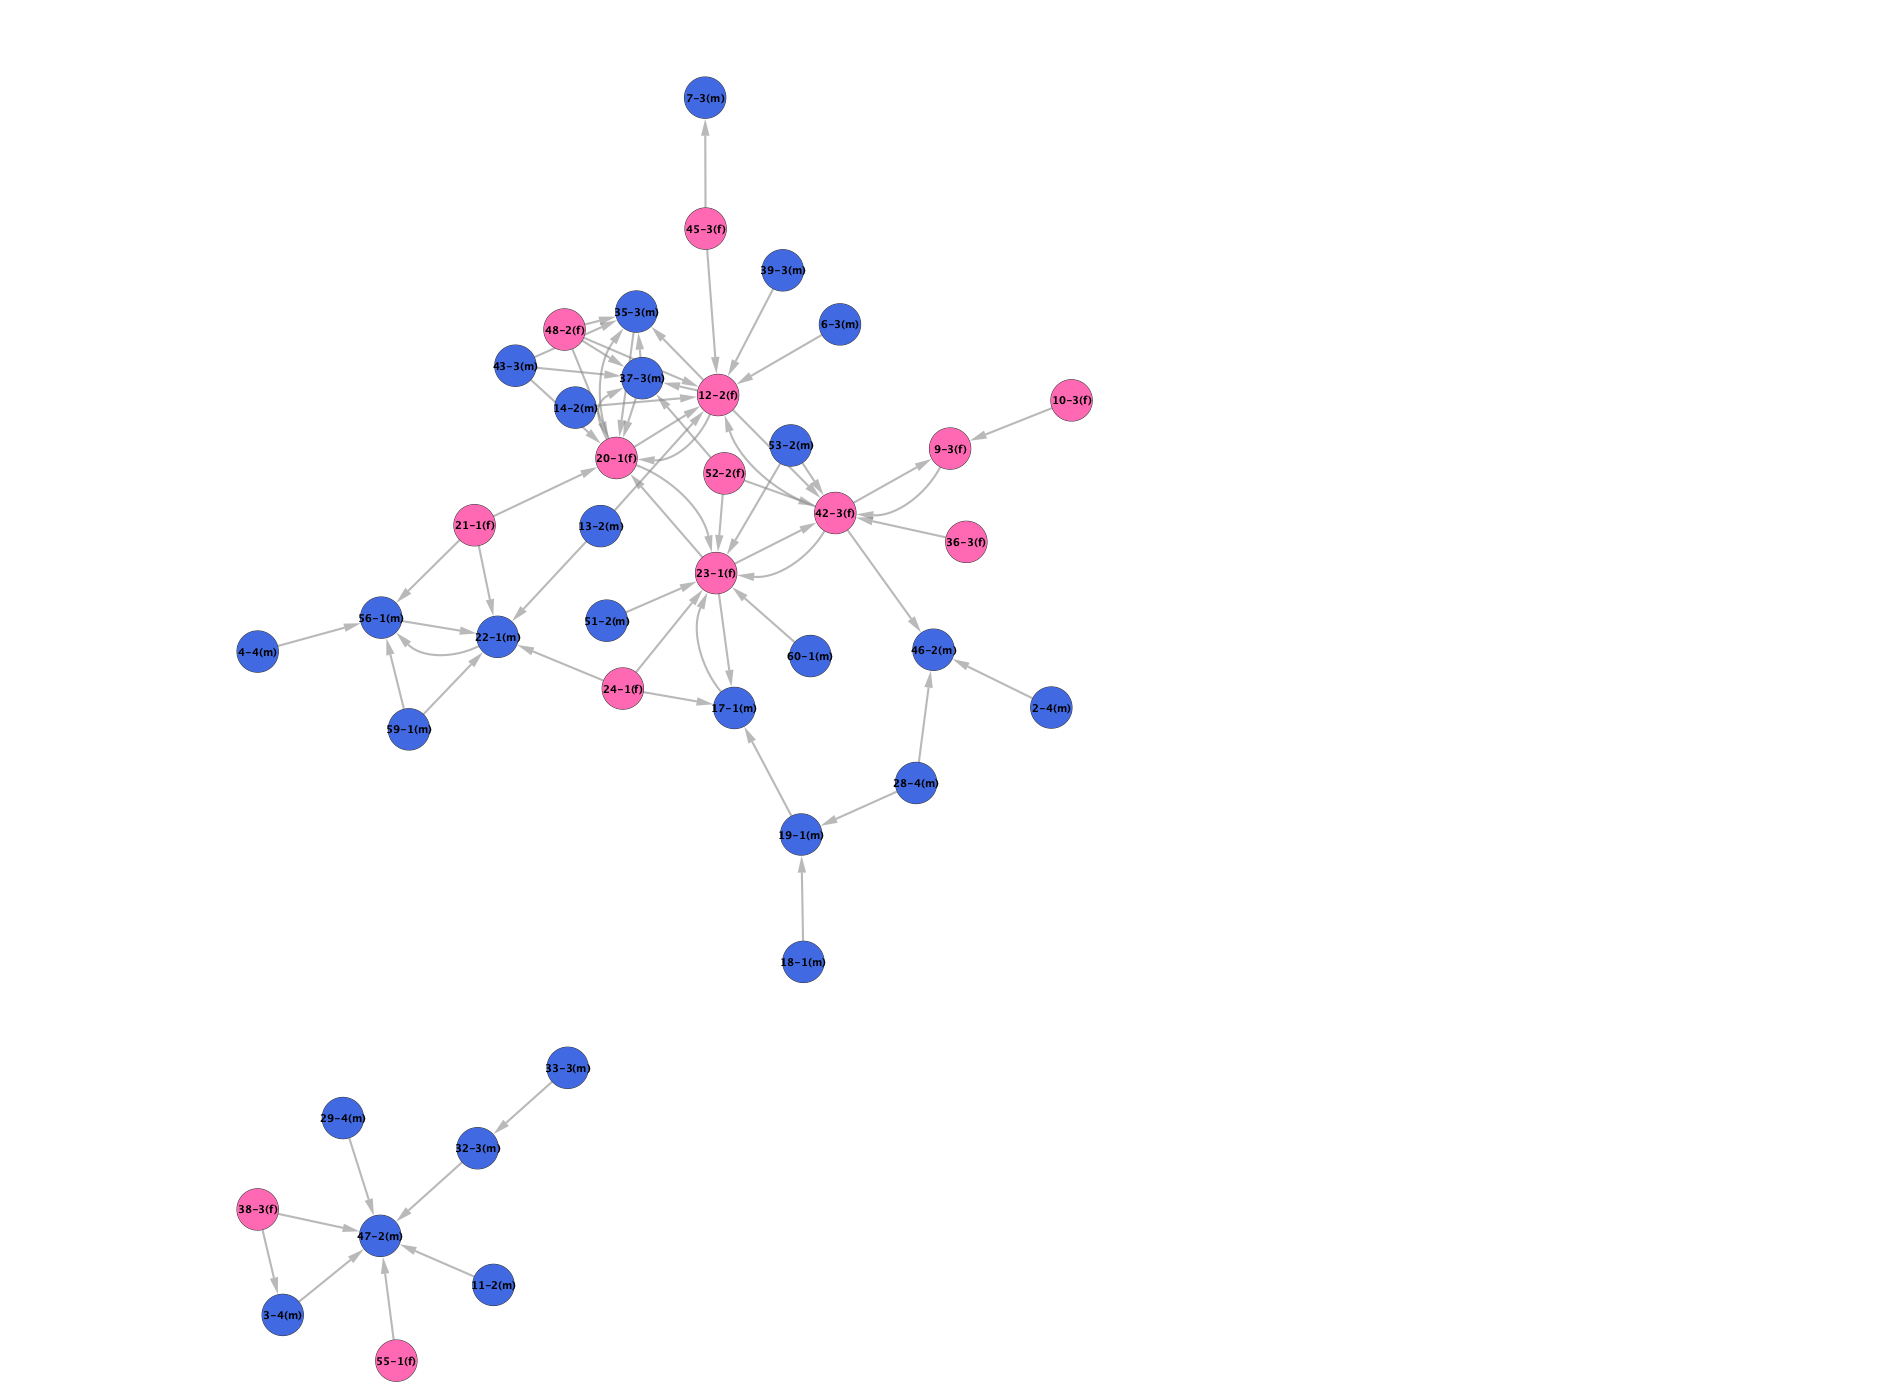
\includegraphics[width=0.95\linewidth]{fig/network_after.png}
\caption{Afterネットワーク（6ヶ月後）．ノード色は性別を示す（ピンク：女性，青：男性）．矢印は友人関係の方向を表す．}
\label{fig:network_after}
\end{figure}
